

% IEEEtran V1.7 and later provides for these CLASSINPUT macros to allow the
% user to reprogram some IEEEtran.cls defaults if needed. These settings
% override the internal defaults of IEEEtran.cls regardless of which class
% options are used. Do not use these unless you have good reason to do so as
% they can result in nonIEEE compliant documents. User beware. ;)
%
%\newcommand{\CLASSINPUTbaselinestretch}{1.0} % baselinestretch
%\newcommand{\CLASSINPUTinnersidemargin}{1in} % inner side margin
%\newcommand{\CLASSINPUToutersidemargin}{1in} % outer side margin
%\newcommand{\CLASSINPUTtoptextmargin}{1in}   % top text margin
%\newcommand{\CLASSINPUTbottomtextmargin}{1in}% bottom text margin




%
\documentclass[10pt,journal,compsoc]{IEEEtran}
% If IEEEtran.cls has not been installed into the LaTeX system files,
% manually specify the path to it like:
% \documentclass[10pt,journal,compsoc]{../sty/IEEEtran}


% For Computer Society journals, IEEEtran defaults to the use of 
% Palatino/Palladio as is done in IEEE Computer Society journals.
% To go back to Times Roman, you can use this code:
%\renewcommand{\rmdefault}{ptm}\selectfont

\usepackage[boxed]{algorithm2e}
\usepackage{algpseudocode}
\usepackage{fullpage}
\usepackage{verbatim}
\usepackage{amsmath}
 \usepackage{booktabs}
\usepackage{subfigure}
\usepackage{graphics}
\usepackage[dvips]{graphicx}
\graphicspath{ {images/}}

% Some very useful LaTeX packages include:
% (uncomment the ones you want to load)



% *** MISC UTILITY PACKAGES ***
%
%\usepackage{ifpdf}
% Heiko Oberdiek's ifpdf.sty is very useful if you need conditional
% compilation based on whether the output is pdf or dvi.
% usage:
% \ifpdf
%   % pdf code
% \else
%   % dvi code
% \fi
% The latest version of ifpdf.sty can be obtained from:
% http://www.ctan.org/tex-archive/macros/latex/contrib/oberdiek/
% Also, note that IEEEtran.cls V1.7 and later provides a builtin
% \ifCLASSINFOpdf conditional that works the same way.
% When switching from latex to pdflatex and vice-versa, the compiler may
% have to be run twice to clear warning/error messages.


% *** CITATION PACKAGES ***
%
\ifCLASSOPTIONcompsoc
  % IEEE Computer Society needs nocompress option
  % requires cite.sty v4.0 or later (November 2003)
  \usepackage[nocompress]{cite}
\else
  % normal IEEE
  \usepackage{cite}
\fi
% cite.sty was written by Donald Arseneau
% V1.6 and later of IEEEtran pre-defines the format of the cite.sty package
% \cite{} output to follow that of IEEE. Loading the cite package will
% result in citation numbers being automatically sorted and properly
% "compressed/ranged". e.g., [1], [9], [2], [7], [5], [6] without using
% cite.sty will become [1], [2], [5]--[7], [9] using cite.sty. cite.sty's
% \cite will automatically add leading space, if needed. Use cite.sty's
% noadjust option (cite.sty V3.8 and later) if you want to turn this off
% such as if a citation ever needs to be enclosed in parenthesis.
% cite.sty is already installed on most LaTeX systems. Be sure and use
% version 5.0 (2009-03-20) and later if using hyperref.sty.
% The latest version can be obtained at:
% http://www.ctan.org/tex-archive/macros/latex/contrib/cite/
% The documentation is contained in the cite.sty file itself.
%
% Note that some packages require special options to format as the Computer
% Society requires. In particular, Computer Society  papers do not use
% compressed citation ranges as is done in typical IEEE papers
% (e.g., [1]-[4]). Instead, they list every citation separately in order
% (e.g., [1], [2], [3], [4]). To get the latter we need to load the cite
% package with the nocompress option which is supported by cite.sty v4.0
% and later.



% *** GRAPHICS RELATED PACKAGES ***
%
\ifCLASSINFOpdf
  % \usepackage[pdftex]{graphicx}
  % declare the path(s) where your graphic files are
  % \graphicspath{{../pdf/}{../jpeg/}}
  % and their extensions so you won't have to specify these with
  % every instance of \includegraphics
  % \DeclareGraphicsExtensions{.pdf,.jpeg,.png}
\else
  % or other class option (dvipsone, dvipdf, if not using dvips). graphicx
  % will default to the driver specified in the system graphics.cfg if no
  % driver is specified.
  % \usepackage[dvips]{graphicx}
  % declare the path(s) where your graphic files are
  % \graphicspath{{../eps/}}
  % and their extensions so you won't have to specify these with
  % every instance of \includegraphics
  % \DeclareGraphicsExtensions{.eps}
\fi
% graphicx was written by David Carlisle and Sebastian Rahtz. It is
% required if you want graphics, photos, etc. graphicx.sty is already
% installed on most LaTeX systems. The latest version and documentation
% can be obtained at: 
% http://www.ctan.org/tex-archive/macros/latex/required/graphics/
% Another good source of documentation is "Using Imported Graphics in
% LaTeX2e" by Keith Reckdahl which can be found at:
% http://www.ctan.org/tex-archive/info/epslatex/
%
% latex, and pdflatex in dvi mode, support graphics in encapsulated
% postscript (.eps) format. pdflatex in pdf mode supports graphics
% in .pdf, .jpeg, .png and .mps (metapost) formats. Users should ensure
% that all non-photo figures use a vector format (.eps, .pdf, .mps) and
% not a bitmapped formats (.jpeg, .png). IEEE frowns on bitmapped formats
% which can result in "jaggedy"/blurry rendering of lines and letters as
% well as large increases in file sizes.
%
% You can find documentation about the pdfTeX application at:
% http://www.tug.org/applications/pdftex


% *** MATH PACKAGES ***
%
%\usepackage[cmex10]{amsmath}
% A popular package from the American Mathematical Society that provides
% many useful and powerful commands for dealing with mathematics. If using
% it, be sure to load this package with the cmex10 option to ensure that
% only type 1 fonts will utilized at all point sizes. Without this option,
% it is possible that some math symbols, particularly those within
% footnotes, will be rendered in bitmap form which will result in a
% document that can not be IEEE Xplore compliant!
%
% Also, note that the amsmath package sets \interdisplaylinepenalty to 10000
% thus preventing page breaks from occurring within multiline equations. Use:
%\interdisplaylinepenalty=2500
% after loading amsmath to restore such page breaks as IEEEtran.cls normally
% does. amsmath.sty is already installed on most LaTeX systems. The latest
% version and documentation can be obtained at:
% http://www.ctan.org/tex-archive/macros/latex/required/amslatex/math/


% *** SPECIALIZED LIST PACKAGES ***
%\usepackage{acronym}
% acronym.sty was written by Tobias Oetiker. This package provides tools for
% managing documents with large numbers of acronyms. (You don't *have* to
% use this package - unless you have a lot of acronyms, you may feel that
% such package management of them is bit of an overkill.)
% Do note that the acronym environment (which lists acronyms) will have a
% problem when used under IEEEtran.cls because acronym.sty relies on the
% description list environment - which IEEEtran.cls has customized for
% producing IEEE style lists. A workaround is to declared the longest
% label width via the IEEEtran.cls \IEEEiedlistdecl global control:
%
% \renewcommand{\IEEEiedlistdecl}{\IEEEsetlabelwidth{SONET}}
% \begin{acronym}
%
% \end{acronym}
% \renewcommand{\IEEEiedlistdecl}{\relax}% remember to reset \IEEEiedlistdecl
%
% instead of using the acronym environment's optional argument.
% The latest version and documentation can be obtained at:
% http://www.ctan.org/tex-archive/macros/latex/contrib/acronym/


%\usepackage{algorithmic}
% algorithmic.sty was written by Peter Williams and Rogerio Brito.
% This package provides an algorithmic environment fo describing algorithms.
% You can use the algorithmic environment in-text or within a figure
% environment to provide for a floating algorithm. Do NOT use the algorithm
% floating environment provided by algorithm.sty (by the same authors) or
% algorithm2e.sty (by Christophe Fiorio) as IEEE does not use dedicated
% algorithm float types and packages that provide these will not provide
% correct IEEE style captions. The latest version and documentation of
% algorithmic.sty can be obtained at:
% http://www.ctan.org/tex-archive/macros/latex/contrib/algorithms/
% There is also a support site at:
% http://algorithms.berlios.de/index.html
% Also of interest may be the (relatively newer and more customizable)
% algorithmicx.sty package by Szasz Janos:
% http://www.ctan.org/tex-archive/macros/latex/contrib/algorithmicx/


% *** ALIGNMENT PACKAGES ***
%
%\usepackage{array}
% Frank Mittelbach's and David Carlisle's array.sty patches and improves
% the standard LaTeX2e array and tabular environments to provide better
% appearance and additional user controls. As the default LaTeX2e table
% generation code is lacking to the point of almost being broken with
% respect to the quality of the end results, all users are strongly
% advised to use an enhanced (at the very least that provided by array.sty)
% set of table tools. array.sty is already installed on most systems. The
% latest version and documentation can be obtained at:
% http://www.ctan.org/tex-archive/macros/latex/required/tools/


%\usepackage{mdwmath}
%\usepackage{mdwtab}
% Also highly recommended is Mark Wooding's extremely powerful MDW tools,
% especially mdwmath.sty and mdwtab.sty which are used to format equations
% and tables, respectively. The MDWtools set is already installed on most
% LaTeX systems. The lastest version and documentation is available at:
% http://www.ctan.org/tex-archive/macros/latex/contrib/mdwtools/


% IEEEtran contains the IEEEeqnarray family of commands that can be used to
% generate multiline equations as well as matrices, tables, etc., of high
% quality.


%\usepackage{eqparbox}
% Also of notable interest is Scott Pakin's eqparbox package for creating
% (automatically sized) equal width boxes - aka "natural width parboxes".
% Available at:
% http://www.ctan.org/tex-archive/macros/latex/contrib/eqparbox/


% *** SUBFIGURE PACKAGES ***
%\ifCLASSOPTIONcompsoc
%  \usepackage[caption=false,font=footnotesize,labelfont=sf,textfont=sf]{subfig}
%\else
%  \usepackage[caption=false,font=footnotesize]{subfig}
%\fi
% subfig.sty, written by Steven Douglas Cochran, is the modern replacement
% for subfigure.sty, the latter of which is no longer maintained and is
% incompatible with some LaTeX packages including fixltx2e. However,
% subfig.sty requires and automatically loads Axel Sommerfeldt's caption.sty
% which will override IEEEtran.cls' handling of captions and this will result
% in non-IEEE style figure/table captions. To prevent this problem, be sure
% and invoke subfig.sty's "caption=false" package option (available since
% subfig.sty version 1.3, 2005/06/28) as this is will preserve IEEEtran.cls
% handling of captions.
% Note that the Computer Society format requires a sans serif font rather
% than the serif font used in traditional IEEE formatting and thus the need
% to invoke different subfig.sty package options depending on whether
% compsoc mode has been enabled.
%
% The latest version and documentation of subfig.sty can be obtained at:
% http://www.ctan.org/tex-archive/macros/latex/contrib/subfig/


% *** FLOAT PACKAGES ***
%
%\usepackage{fixltx2e}
% fixltx2e, the successor to the earlier fix2col.sty, was written by
% Frank Mittelbach and David Carlisle. This package corrects a few problems
% in the LaTeX2e kernel, the most notable of which is that in current
% LaTeX2e releases, the ordering of single and double column floats is not
% guaranteed to be preserved. Thus, an unpatched LaTeX2e can allow a
% single column figure to be placed prior to an earlier double column
% figure. The latest version and documentation can be found at:
% http://www.ctan.org/tex-archive/macros/latex/base/


%\usepackage{stfloats}
% stfloats.sty was written by Sigitas Tolusis. This package gives LaTeX2e
% the ability to do double column floats at the bottom of the page as well
% as the top. (e.g., "\begin{figure*}[!b]" is not normally possible in
% LaTeX2e). It also provides a command:
%\fnbelowfloat
% to enable the placement of footnotes below bottom floats (the standard
% LaTeX2e kernel puts them above bottom floats). This is an invasive package
% which rewrites many portions of the LaTeX2e float routines. It may not work
% with other packages that modify the LaTeX2e float routines. The latest
% version and documentation can be obtained at:
% http://www.ctan.org/tex-archive/macros/latex/contrib/sttools/
% Do not use the stfloats baselinefloat ability as IEEE does not allow
% \baselineskip to stretch. Authors submitting work to the IEEE should note
% that IEEE rarely uses double column equations and that authors should try
% to avoid such use. Do not be tempted to use the cuted.sty or midfloat.sty
% packages (also by Sigitas Tolusis) as IEEE does not format its papers in
% such ways.
% Do not attempt to use stfloats with fixltx2e as they are incompatible.
% Instead, use Morten Hogholm'a dblfloatfix which combines the features
% of both fixltx2e and stfloats:
%
% \usepackage{dblfloatfix}
% The latest version can be found at:
% http://www.ctan.org/tex-archive/macros/latex/contrib/dblfloatfix/


%\ifCLASSOPTIONcaptionsoff
%  \usepackage[nomarkers]{endfloat}
% \let\MYoriglatexcaption\caption
% \renewcommand{\caption}[2][\relax]{\MYoriglatexcaption[#2]{#2}}
%\fi
% endfloat.sty was written by James Darrell McCauley, Jeff Goldberg and 
% Axel Sommerfeldt. This package may be useful when used in conjunction with 
% IEEEtran.cls'  captionsoff option. Some IEEE journals/societies require that
% submissions have lists of figures/tables at the end of the paper and that
% figures/tables without any captions are placed on a page by themselves at
% the end of the document. If needed, the draftcls IEEEtran class option or
% \CLASSINPUTbaselinestretch interface can be used to increase the line
% spacing as well. Be sure and use the nomarkers option of endfloat to
% prevent endfloat from "marking" where the figures would have been placed
% in the text. The two hack lines of code above are a slight modification of
% that suggested by in the endfloat docs (section 8.4.1) to ensure that
% the full captions always appear in the list of figures/tables - even if
% the user used the short optional argument of \caption[]{}.
% IEEE papers do not typically make use of \caption[]'s optional argument,
% so this should not be an issue. A similar trick can be used to disable
% captions of packages such as subfig.sty that lack options to turn off
% the subcaptions:
% For subfig.sty:
% \let\MYorigsubfloat\subfloat
% \renewcommand{\subfloat}[2][\relax]{\MYorigsubfloat[]{#2}}
% However, the above trick will not work if both optional arguments of
% the \subfloat command are used. Furthermore, there needs to be a
% description of each subfigure *somewhere* and endfloat does not add
% subfigure captions to its list of figures. Thus, the best approach is to
% avoid the use of subfigure captions (many IEEE journals avoid them anyway)
% and instead reference/explain all the subfigures within the main caption.
% The latest version of endfloat.sty and its documentation can obtained at:
% http://www.ctan.org/tex-archive/macros/latex/contrib/endfloat/
%
% The IEEEtran \ifCLASSOPTIONcaptionsoff conditional can also be used
% later in the document, say, to conditionally put the References on a 
% page by themselves.


% *** PDF, URL AND HYPERLINK PACKAGES ***
%
%\usepackage{url}
% url.sty was written by Donald Arseneau. It provides better support for
% handling and breaking URLs. url.sty is already installed on most LaTeX
% systems. The latest version and documentation can be obtained at:
% http://www.ctan.org/tex-archive/macros/latex/contrib/url/
% Basically, \url{my_url_here}.


% NOTE: PDF thumbnail features are not required in IEEE papers
%       and their use requires extra complexity and work.
%\ifCLASSINFOpdf
%  \usepackage[pdftex]{thumbpdf}
%\else
%  \usepackage[dvips]{thumbpdf}
%\fi
% thumbpdf.sty and its companion Perl utility were written by Heiko Oberdiek.
% It allows the user a way to produce PDF documents that contain fancy
% thumbnail images of each of the pages (which tools like acrobat reader can
% utilize). This is possible even when using dvi->ps->pdf workflow if the
% correct thumbpdf driver options are used. thumbpdf.sty incorporates the
% file containing the PDF thumbnail information (filename.tpm is used with
% dvips, filename.tpt is used with pdftex, where filename is the base name of
% your tex document) into the final ps or pdf output document. An external
% utility, the thumbpdf *Perl script* is needed to make these .tpm or .tpt
% thumbnail files from a .ps or .pdf version of the document (which obviously
% does not yet contain pdf thumbnails). Thus, one does a:
% 
% thumbpdf filename.pdf 
%
% to make a filename.tpt, and:
%
% thumbpdf --mode dvips filename.ps
%
% to make a filename.tpm which will then be loaded into the document by
% thumbpdf.sty the NEXT time the document is compiled (by pdflatex or
% latex->dvips->ps2pdf). Users must be careful to regenerate the .tpt and/or
% .tpm files if the main document changes and then to recompile the
% document to incorporate the revised thumbnails to ensure that thumbnails
% match the actual pages. It is easy to forget to do this!
% 
% Unix systems come with a Perl interpreter. However, MS Windows users
% will usually have to install a Perl interpreter so that the thumbpdf
% script can be run. The Ghostscript PS/PDF interpreter is also required.
% See the thumbpdf docs for details. The latest version and documentation
% can be obtained at.
% http://www.ctan.org/tex-archive/support/thumbpdf/


% NOTE: PDF hyperlink and bookmark features are not required in IEEE
%       papers and their use requires extra complexity and work.
% *** IF USING HYPERREF BE SURE AND CHANGE THE EXAMPLE PDF ***
% *** TITLE/SUBJECT/AUTHOR/KEYWORDS INFO BELOW!!           ***
\newcommand\MYhyperrefoptions{bookmarks=true,bookmarksnumbered=true,
pdfpagemode={UseOutlines},plainpages=false,pdfpagelabels=true,
colorlinks=true,linkcolor={black},citecolor={black},urlcolor={black},
pdftitle={Bare Demo of IEEEtran.cls for Computer Society Journals},%<!CHANGE!
pdfsubject={Typesetting},%<!CHANGE!
pdfauthor={Michael D. Shell},%<!CHANGE!
pdfkeywords={Computer Society, IEEEtran, journal, LaTeX, paper,
             template}}%<^!CHANGE!
%\ifCLASSINFOpdf
%\usepackage[\MYhyperrefoptions,pdftex]{hyperref}
%\else
%\usepackage[\MYhyperrefoptions,breaklinks=true,dvips]{hyperref}
%\usepackage{breakurl}
%\fi
% One significant drawback of using hyperref under DVI output is that the
% LaTeX compiler cannot break URLs across lines or pages as can be done
% under pdfLaTeX's PDF output via the hyperref pdftex driver. This is
% probably the single most important capability distinction between the
% DVI and PDF output. Perhaps surprisingly, all the other PDF features
% (PDF bookmarks, thumbnails, etc.) can be preserved in
% .tex->.dvi->.ps->.pdf workflow if the respective packages/scripts are
% loaded/invoked with the correct driver options (dvips, etc.). 
% As most IEEE papers use URLs sparingly (mainly in the references), this
% may not be as big an issue as with other publications.
%
% That said, Vilar Camara Neto created his breakurl.sty package which
% permits hyperref to easily break URLs even in dvi mode.
% Note that breakurl, unlike most other packages, must be loaded
% AFTER hyperref. The latest version of breakurl and its documentation can
% be obtained at:
% http://www.ctan.org/tex-archive/macros/latex/contrib/breakurl/
% breakurl.sty is not for use under pdflatex pdf mode.
%
% The advanced features offer by hyperref.sty are not required for IEEE
% submission, so users should weigh these features against the added
% complexity of use.
% The package options above demonstrate how to enable PDF bookmarks
% (a type of table of contents viewable in Acrobat Reader) as well as
% PDF document information (title, subject, author and keywords) that is
% viewable in Acrobat reader's Document_Properties menu. PDF document
% information is also used extensively to automate the cataloging of PDF
% documents. The above set of options ensures that hyperlinks will not be
% colored in the text and thus will not be visible in the printed page,
% but will be active on "mouse over". USING COLORS OR OTHER HIGHLIGHTING
% OF HYPERLINKS CAN RESULT IN DOCUMENT REJECTION BY THE IEEE, especially if
% these appear on the "printed" page. IF IN DOUBT, ASK THE RELEVANT
% SUBMISSION EDITOR. You may need to add the option hypertexnames=false if
% you used duplicate equation numbers, etc., but this should not be needed
% in normal IEEE work.
% The latest version of hyperref and its documentation can be obtained at:
% http://www.ctan.org/tex-archive/macros/latex/contrib/hyperref/


% *** Do not adjust lengths that control margins, column widths, etc. ***
% *** Do not use packages that alter fonts (such as pslatex).         ***
% There should be no need to do such things with IEEEtran.cls V1.6 and later.
% (Unless specifically asked to do so by the journal or conference you plan
% to submit to, of course. )


% correct bad hyphenation here
\hyphenation{op-tical net-works semi-conduc-tor}


\begin{document}
%
% paper title
% Titles are generally capitalized except for words such as a, an, and, as,
% at, but, by, for, in, nor, of, on, or, the, to and up, which are usually
% not capitalized unless they are the first or last word of the title.
% Linebreaks \\ can be used within to get better formatting as desired.
% Do not put math or special symbols in the title.
\title{Finding Influential People from a Historical News Repository}
%
%
% author names and IEEE memberships
% note positions of commas and nonbreaking spaces ( ~ ) LaTeX will not break
% a structure at a ~ so this keeps an author's name from being broken across
% two lines.
% use \thanks{} to gain access to the first footnote area
% a separate \thanks must be used for each paragraph as LaTeX2e's \thanks
% was not built to handle multiple paragraphs
%
%
%\IEEEcompsocitemizethanks is a special \thanks that produces the bulleted
% lists the Computer Society journals use for "first footnote" author
% affiliations. Use \IEEEcompsocthanksitem which works much like \item
% for each affiliation group. When not in compsoc mode,
% \IEEEcompsocitemizethanks becomes like \thanks and
% \IEEEcompsocthanksitem becomes a line break with idention. This
% facilitates dual compilation, although admittedly the differences in the
% desired content of \author between the different types of papers makes a
% one-size-fits-all approach a daunting prospect. For instance, compsoc 
% journal papers have the author affiliations above the "Manuscript
% received ..."  text while in non-compsoc journals this is reversed. Sigh.


\author{Aayushee~Gupta, Hamonti~Dutta, Lipika~Dey, Srikanta~Bedathur}
%\author{Michael~Shell,~\IEEEmembership{Member,~IEEE,}
%        John~Doe,~\IEEEmembership{Fellow,~OSA,}
%        and~Jane~Doe,~\IEEEmembership{Life~Fellow,~IEEE}
%\IEEEcompsocitemizethanks{\IEEEcompsocthanksitem M. Shell is with the Department
%of Electrical and Computer Engineering, Georgia Institute of Technology, Atlanta,
%GA, 30332.\protect\\
%% note need leading \protect in front of \\ to get a newline within \thanks as
%% \\ is fragile and will error, could use \hfil\break instead.
%E-mail: see http://www.michaelshell.org/contact.html
%\IEEEcompsocthanksitem J. Doe and J. Doe are with Anonymous University.}% <-this % stops a space
%\thanks{Manuscript received April 19, 2005; revised September 17, 2014.}}

% note the % following the last \IEEEmembership and also \thanks - 
% these prevent an unwanted space from occurring between the last author name
% and the end of the author line. i.e., if you had this:
% 
% \author{....lastname \thanks{...} \thanks{...} }
%                     ^------------^------------^----Do not want these spaces!
%
% a space would be appended to the last name and could cause every name on that
% line to be shifted left slightly. This is one of those "LaTeX things". For
% instance, "\textbf{A} \textbf{B}" will typeset as "A B" not "AB". To get
% "AB" then you have to do: "\textbf{A}\textbf{B}"
% \thanks is no different in this regard, so shield the last } of each \thanks
% that ends a line with a % and do not let a space in before the next \thanks.
% Spaces after \IEEEmembership other than the last one are OK (and needed) as
% you are supposed to have spaces between the names. For what it is worth,
% this is a minor point as most people would not even notice if the said evil
% space somehow managed to creep in.



% The paper headers IS THIS REQUIRED??
%\markboth{Journal of \LaTeX\ Class Files,~Vol.~13, No.~9, September~2014}%
%{Shell \MakeLowercase{\textit{et al.}}: Bare Advanced Demo of IEEEtran.cls for Journals}
% The only time the second header will appear is for the odd numbered pages
% after the title page when using the twoside option.
% 
% *** Note that you probably will NOT want to include the author's ***
% *** name in the headers of peer review papers.                   ***
% You can use \ifCLASSOPTIONpeerreview for conditional compilation here if
% you desire.



% The publisher's ID mark at the bottom of the page is less important with
% Computer Society journal papers as those publications place the marks
% outside of the main text columns and, therefore, unlike regular IEEE
% journals, the available text space is not reduced by their presence.
% If you want to put a publisher's ID mark on the page you can do it like
% this:
%\IEEEpubid{0000--0000/00\$00.00~\copyright~2014 IEEE}
% or like this to get the Computer Society new two part style.
%\IEEEpubid{\makebox[\columnwidth]{\hfill 0000--0000/00/\$00.00~\copyright~2014 IEEE}%
%\hspace{\columnsep}\makebox[\columnwidth]{Published by the IEEE Computer Society\hfill}}
% Remember, if you use this you must call \IEEEpubidadjcol in the second
% column for its text to clear the IEEEpubid mark (Computer Society journal
% papers don't need this extra clearance.)



% use for special paper notices
%\IEEEspecialpapernotice{(Invited Paper)}



% for Computer Society papers, we must declare the abstract and index terms
% PRIOR to the title within the \IEEEtitleabstractindextext IEEEtran
% command as these need to go into the title area created by \maketitle.
% As a general rule, do not put math, special symbols or citations
% in the abstract or keywords.
\IEEEtitleabstractindextext{%
\begin{abstract}

 Historical newspaper archives provide a wealth of information. They
are of particular interest to genealogists, historians and scholars
for People Search. In this paper, we design a People Gazetteer from
the noisy OCR text of historical newspapers and identify ``influential"
people from it. A People Gazetteer is a dictionary of personal names;
each entry of the gazetteer is a tuple containing a person name and a
list of articles in which his name occurs along with the corresponding
topic associated with each article.

To build the People Gazetteer, we first spell correct the noisy text
using an edit distance based algorithm. A novel N-gram based
evaluation algorithm is designed for measuring the performance of the
spell corrector. Next, a Named Entity Recognizer is run on the text of
each article to identify person entities and an LDA-based topic
detector to assign categories to articles. To identify influential
people across each category of People Gazetteer, we define the notion
of an Influential Person Index (IPI) and rank based on it. 

Our corpus is a sample of 14020 OCR newspaper articles (roughly two months' data)
obtained from ``The Sun" newspaper in the Chronicling America project.
We present results on the top-K influential people obtained from our algorithm by varying its parameters and verify results using Wikipedia.
\end{abstract}

% Note that keywords are not normally used for peerreview papers.
\begin{IEEEkeywords}
 Gazetteer, Text Mining, Information Retrieval, OCR, Spelling Correction, Historical data, Influential people detection.
\end{IEEEkeywords}}


% make the title area
\maketitle


% To allow for easy dual compilation without having to reenter the
% abstract/keywords data, the \IEEEtitleabstractindextext text will
% not be used in maketitle, but will appear (i.e., to be "transported")
% here as \IEEEdisplaynontitleabstractindextext when compsoc mode
% is not selected <OR> if conference mode is selected - because compsoc
% conference papers position the abstract like regular (non-compsoc)
% papers do!
\IEEEdisplaynontitleabstractindextext
% \IEEEdisplaynontitleabstractindextext has no effect when using
% compsoc under a non-conference mode.


% For peer review papers, you can put extra information on the cover
% page as needed:
% \ifCLASSOPTIONpeerreview
% \begin{center} \bfseries EDICS Category: 3-BBND \end{center}
% \fi
%
% For peerreview papers, this IEEEtran command inserts a page break and
% creates the second title. It will be ignored for other modes.
\IEEEpeerreviewmaketitle


\ifCLASSOPTIONcompsoc
\IEEEraisesectionheading{\section{Introduction}\label{sec:introduction}}
\else
\section{Introduction}
\label{sec:introduction}
\fi
% Computer Society journal (but not conference!) papers do something unusual
% with the very first section heading (almost always called "Introduction").
% They place it ABOVE the main text! IEEEtran.cls does not automatically do
% this for you, but you can achieve this effect with the provided
% \IEEEraisesectionheading{} command. Note the need to keep any \label that
% is to refer to the section immediately after \section in the above as
% \IEEEraisesectionheading puts \section within a raised box.




% The very first letter is a 2 line initial drop letter followed
% by the rest of the first word in caps (small caps for compsoc).
% 
% form to use if the first word consists of a single letter:
% \IEEEPARstart{A}{demo} file is ....
% 
% form to use if you need the single drop letter followed by
% normal text (unknown if ever used by IEEE):
% \IEEEPARstart{A}{}demo file is ....
% 
% Some journals put the first two words in caps:
% \IEEEPARstart{T}{his demo} file is ....
% 
% Here we have the typical use of a "T" for an initial drop letter
% and "HIS" in caps to complete the first word.
\IEEEPARstart{A}{n}
 important use of historical newspapers is for People Search\cite{BilenkoMCRF03,Friedman_92}) -- for example, to find important people and track the timelines of news articles related to them. Several websites like Genealogy Bank\footnote{http://www.genealogybank.com/gbnk/}, FamilySearch\footnote{https://familysearch.org/}, Newspaper Archives\footnote{http://newspaperarchive.com/}, Ancestry\footnote{http://www.ancestry.com/} provide people search service that include obituaries, birth and death lists, newspaper articles, military records, Revolutionary and Civil War pension requests, census records, land grants and other forms of petitions.
% SHOULD I INCLUDE BOTH IMAGES OF ONLINE SEARCH TOOLS HERE?
% Figure~\ref{figSearch} shows two such tools available online.

To the best of our knowledge, the problem of finding \emph{influential} people from historic newspaper archives has not been studied before. This exercise, however, opens up a wide range of possibilities -- for example, news articles related to the influential person can also be linked to a Wikipedia page entry to find out relevant details or build influential people networks that can learn about entities involved in historical events.

% You must have at least 2 lines in the paragraph with the drop letter
% (should never be an issue)


\section{Problem Description}
\label{problem}

The goal of this research is to find and rank influential people in historical newspaper OCR archives.
  
 An influential person can be defined as ``a person whose actions and opinions strongly influence a course of events". This allows us to link an influential person with a list of articles that s/he occurs in.
 A person may also be considered influential if s/he gets talked about frequently in news articles. The problem can be also be phrased as identifying and ranking \emph{popular} people in the news domain. 
 ``Popularity" has been defined in other domains by counting number of votes, tweets, citations and followers \cite{cheng2014can} but similar measures are not applicable in a newspaper setting where only the newspaper articles mentioning multiple people names are available.  
 
We divide the the problem of finding influential people into the following subproblems:
\begin{itemize}
\item \textbf{Problem 1: } Spell Correction and Cleaning of OCR text
\item \textbf{Problem 2: } Development of a People Gazetteer -- develop an organized structure in order to ease the process of identification of influential people.
\item \textbf{Problem 3: } Influential People Identification -- define the criteria for identifying and ranking people as ``influential".
\end{itemize}

\begin{figure*}
\centering
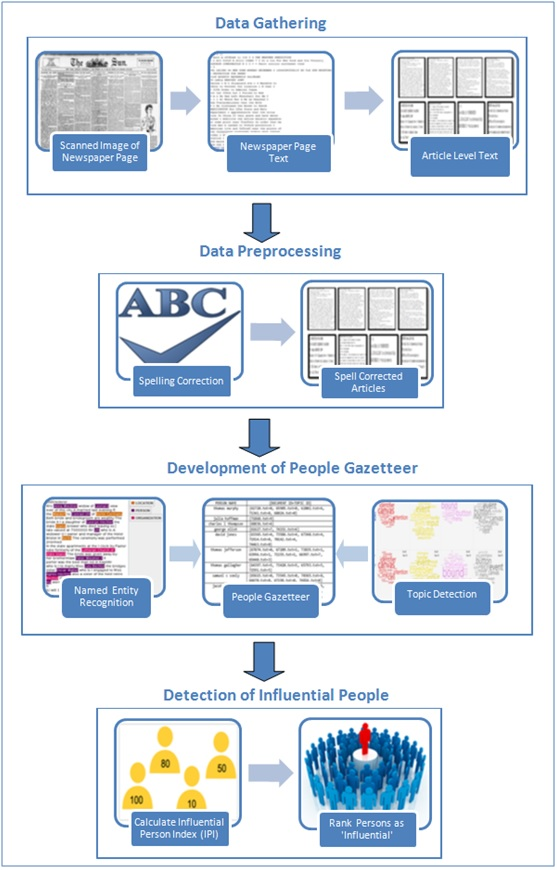
\includegraphics[width=0.65\textwidth, height=0.6\textheight]{framework4}
\caption{Research Framework showing components of proposed solution}
\label{fig:framework}
\end{figure*} 



\section{ Novel Research Contributions}
\label{intro:rc}
The paper has the following novel contributions:
\begin{enumerate}
\item A new algorithm for \emph{evaluation} of the performance of the spelling correction algorithm is presented. 
\item Development of the People Gazetteer -- an organized dictionary of people names and a list of articles in which the name occurs along with the corresponding topic of each article to facilitate identification of influential people.
\item Define an Influential Person Index (IPI) and metrics for its calculation in order to identify and rank influential people. Case studies of the top-K influential people detected are also discussed and verified with Wikipedia data. 

\end{enumerate}

\section{Related Work}
\label{influential:rw}


Influential people detection has been mostly done in the field of social networks, marketing and diffusion research.
\cite{kempe2003maximizing} work on choosing the most influential set of nodes  in a social network in order to maximize user influence in the network. They consider spread of influence from an influential node cascading through a network which further influences other neighborhood nodes but we do not consider the case of a network of connected person entities in our research where influence score of a person entity could be influenced by that of its neighboring person entity nodes. We consider each person entity connected with a list of articles of its occurrence instead and measure the person entity's influence score by finding the effect of influence of each article in that list.
 

\cite{lerman2010using} define popularity of a news story in terms of number of reader votes received by it and predict popularity of a news story over time based on voting history and the probability that a user seeing a story at specific position in a list will vote on it. 
A more relevant work regarding detection of influential people is presented in \cite{agarwal2008identifying} where influential bloggers are identified on a blog site. Influence of each blogger is quantified by taking maximum of the influence scores of each blog posted by a blogger. The influence score of each blog is calculated using parameters of importance in a blogsite like number of posts that refer to the blog, number of comments on the blog, number of other posts that the blog refers to and length of the blog. Influential blogger categories are also created based on the temporal patterns of blog posting by bloggers. 

\cite{cha2010measuring} describe another set of measures for detection of top influential users on Twitter using number of retweets, mentions and followers for an individual. They perform ranking based on each measure separately and use Spearman's rank correlation coefficient to find correlation among ranks and effect of each measure contributing to a person's influence. The influence ranks of topmost influential users on Twitter are presented across various topics as well as time.

In the above mentioned works, although the problem description matches with our research problem but the parameters defined to measure influence or popularity cannot be directly used in the newspaper environment. 

\section{Dataset Description}
The dataset has been taken from Chronicling America.
\footnote{\texttt{http://chroniclingamerica.loc.gov/}} is an
initiative of the National Endowment for Humanities (NEH) and the
Library of Congress (LC) whose goal is to develop an online,
searchable database of historically significant newspapers between
1836 and 1922. 
In order to make a newspaper available for searching on the Internet,
the following processes used in \cite{dutta2011learning} must take place: (1) the microfilm copy or
paper original is scanned; (2) master and Web image files are
generated; (3) metadata is assigned for each page to improve the
search capability of the newspaper; (4) OCR software is run over high
resolution images to create searchable full text and (5) OCR text,
images, and metadata are imported into a digital library software
program. The scanned newspaper holdings of the NYPL offers a wealth of
data and opinion for researchers and historians.
The newspapers are scanned on a page-by-page basis and article level
segmentation is poor or non-existent; the OCR scanning process is far
from perfect and the documents generated from it contains a large
amount of garbled text.

\begin{figure*}
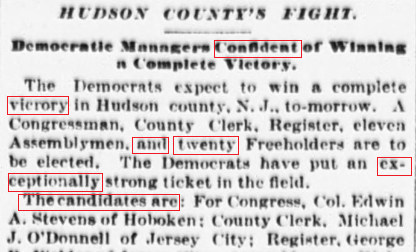
\includegraphics[scale=0.75]{originalimage}
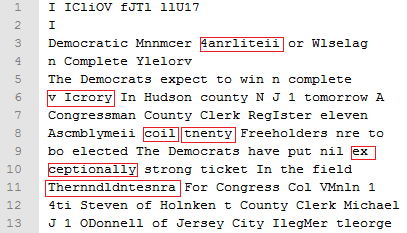
\includegraphics[scale=0.80]{ocr}
\caption{Scanned Image of a Newspaper article (left) and its OCR raw text (right)}
\label{figure:1}
\end{figure*}

\subsection{Data Characteristics}
An individual OCR text article has at least one or more of the following types of spelling errors:



\begin{itemize}
 \item \textbf{Real word errors}	 include words that are spelled correctly in the OCR text but still incorrect when compared to the original newspaper article image. For example: In Figure~\ref{figure:1}, the word ``coil"  has been correctly spelled in the OCR text  but should have been ``and" according to the original newspaper article. 
 \item \textbf{Non-real word} errors include words that have been misspelled due to some insertion, deletion, substitution or transposition of characters from a word. For eg. In Figure~\ref{figure:1}, the word ``tnenty" in the OCR text has a substitution error (`n' should have been `w') which is actually ``twenty" according to the original newspaper article.
 \item \textbf{Non-word errors} include words that have been spelled incorrectly and are a combination of alphabets and numerical characters. For example: In Figure~\ref{figure:1}, the word ``4anrliteii" which is a combination of alphabets and number and should have been ``confident" as per the original newspaper article.
\item \textbf{New Line errors} include words that are separated by hyphens where part of a word is written on one text line and remaining part in the next line. For example: In Figure~\ref{figure:1}, the word ``ex-ceptionally" where ``ex" occurs on one line while ``ceptionally" in the next and due to no punctuation in the text, they are treated as separate words in OCR text.
\item \textbf{Word Split and Join errors} include words that either get split into one of more parts or some words in a sentence get joined to a make a single word. For example: In Figure~\ref{figure:1}, the word ``Thernndldntesnra" in the OCR text is actually a combination of three words ``The candidates are" while the words ``v Icrory" are actually equivalent to a single word ``victory" when compared with the original news article.
\end{itemize} 

\subsection{Data Statistics}
The OCR text available from Chronicling America website is on a page by page level and no article level segmentation is provided. OCR text dataset is therefore, taken from a PostgreSQL database where article level segmentation of page-level OCR text from Chronicling America is available for two months of articles of ``The Sun" newspaper from November-December 1894 consisting of 14020 news articles with a total of 8,403,844 tokens. The newspaper database ER diagram \footnote{https://power.ldeo.columbia.edu/twiki/pub/Incubator/BodhiDBDesign/Final ERD.pdf }
is used to extract the required articles text from the database by dumping complete dataset and extracting individual articles linetext based on their unique ID. The individual text articles generated from the database do not have any punctuation and contain a large amount of garbled text containing above mentioned OCR errors.


\subsection{Data Preprocessing}
The garbled OCR text makes data preprocessing mandatory before application of any text mining algorithms. We,therefore, use edit distance algorithm based on Levenshtein distance to perform spelling correction on the OCR text articles. The algorithm is chosen because of its speed and ability to correct OCR errors compared to the n-gram approach \cite{chattopadhyaya2013fast}. Our edit distance algorithm also uses an enhanced dictionary for look up to give significance to personal names spelling correction in the dataset. 

%SHOULD RESULTS OF SPELLING CORRECTION ECTION BE ADDED HERE? PNDR AND ACCURACY?




\section{Development of People Gazetteer}
\label{chapter:people gazetteer}

People Gazetteer as defined in Section~\ref{sec:introduction} consists of tuples of person names along with list of documents in which they occur and their corresponding topics. It is developed as an organized structure that can facilitate the process of detection of influential persons from the dataset in an efficient and easy way. This section describes the 2-step process of construction of the People Gazetteer by
a) Extraction of person names from the news articles dataset using Named Entity Recognition in  Section~\ref{ner} and
b) Assignment of topics to news articles using LDA topic detection in  Section~\ref{topic detection}.
Output of People gazetteer developed using these steps is presented in Section ~\ref{gaz:result} followed by discussion in Section~\ref{gaz:discussion}

\subsection{Person Named Entity Recognition (PNER)}
\label{ner}


\subsubsection{Definition}
NER (Named Entity Recognition) refers to classification of elements in text into pre-defined categories such as the names of persons, organizations, locations, expressions of times, quantities, monetary values, percentages, etc. 
Person Named Entity Recognition (PNER) can be defined as the process of NER that marks up only person names that occur in the text.

PNER is required in this research so as to extract all person name entities occurring in the complete dataset and identify influential person entities among them through development of the People Gazetteer. 
PNER aids in the development of People Gazetteer by first extracting all person names occurring in the dataset followed by reverse linking of a person with the articles in which he/she occurs.

\subsubsection{Methodology}

The Stanford CRF-NER\footnote{http://nlp.stanford.edu/software/CRF-NER.shtml} is used for PNER in this research. It can perform NER for 3 classes: Person, Organization and Location and is based on linear chain CRF (Conditional Random Field) sequence models. It is trained across several corpora and is fairly robust across multiple domains and even better when compared to some other open source NER systems as illustrated in \cite{rodriquez2012comparison}. According to their results, Stanford NER gave overall the best performance across 2 OCR datasets, and was most effective for PNER when compared with 3 other open source NER systems.


\subsubsection{PNER Results}
\label{ner:results}
\begin{figure*}
  \centering
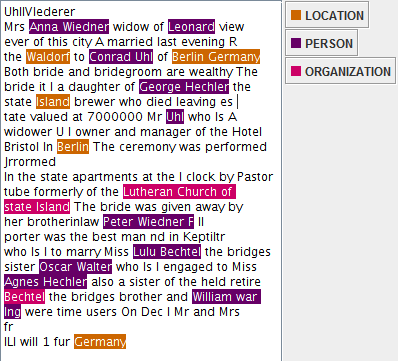
\includegraphics{NER1}
\caption{NER on a sample news article}
\label{figure:sample}
\end{figure*} 




NER on a sample news article from the dataset can be seen in Figure~\ref{figure:sample}.
 Stanford NER recognizes a person's full name as separate names by default which is rectified by combining these multi-term entities into single person entities. For example, the person name ``John Smith" is recognized as two separate person entities which we combine to form a single multi-term person entity.
Person names tagged with ``PERSON" category are stored while running NER on the dataset.
Whenever a multi-term person name (number of terms in the person name must be greater than 1) occurs in a document, the person entity's name along with the document name is stored to obtain tuples of person names with their document lists.
The Stanford NER takes 25 minutes to run on the complete news dataset of 14020 articles extracting a total of 38426 person entities. The output obtained can be seen in Table~\ref{table:Table1} which shows the number of person entities with the corresponding number of documents in which they occur.  

\begin{table*}
  \begin{center}
\begin{tabular}{|l|l|l|}
    \hline
\textbf{No. of Person Entities} & \textbf{No. of articles} \\ \hline
36615                  & 1               \\ \hline
1122                   & 2               \\	\hline
329                    & 3               \\	\hline
123                    & 4               \\	\hline
87                     & 5               \\	\hline
48                     & 6               \\	\hline
29                     & 7               \\	\hline
19                     & 8               \\	\hline
16                     & 9               \\	\hline
5                      & 10              \\	\hline
4                      & 11              \\	\hline
6                      & 12              \\	\hline
4                      & 14              \\	\hline
3                      & 15              \\	\hline
2                      & 16              \\	\hline
1                      & 17              \\	\hline
1                      & 18              \\	\hline
3                      & 19              \\	\hline
1                      & 20              \\	\hline
1                      & 21              \\	\hline
1                      & 22              \\	\hline
1                      & 23              \\	\hline
1                      & 27              \\	\hline
1                      & 29              \\	\hline
1                      & 31              \\	\hline
1                      & 34              \\	\hline
1                      & 35              \\ 	\hline
\end{tabular}
\end{center}
\caption{Table showing output of PNER on 14020 articles}
\label{table:Table1}
\end{table*}


We divide the people entities extracted into following categories so that separate analysis can be done for each category:
\begin{itemize}
 \item \textbf{Marginally Influential}: This category includes all person entities with occurrence in less than 4 news articles. (38066 person entities as calculated from Table~\ref{table:Table1} )
\item \textbf{Medium Influential}: This category includes all person entities with occurrence from 4 to 15 news articles. (344 person entities) 
\item \textbf{Highly Influential} : This category includes all person entities with occurrence in 16 or more news articles. (16 person entities)
\end{itemize}
These categories have been created manually simply based on the number of articles of occurrence of a person entity and do not directly lead to the conclusion of a person entity with large number of articles being influential.


\subsection{Topic Detection}
\label{topic detection}

 Topic models are algorithms for discovering the main topics that occur across a large and otherwise 
unstructured collection of documents and can organize the collection according to the discovered topics.
Here, a topic refers to a set of words which describe what any document is about.
 A topic model examines the set of documents and discovers based on the statistics of the words in each, what the topics might be and what each document's balance of topics is.
Documents are considered as a mixture of topics and each topic a probability distribution over words.
 Topic detection is the process of identifying topics in a document collection using a topic model. A simple example of topic model illustrated by \cite{blei2012probabilistic} can be seen in Figure~\ref{figure:example}.

Topic detection is essential to this research in order to determine the topics of individual news articles that a person entity occurs in so that the person entity can be linked to the documents in which he/she occurs along with their respective topics.

\begin{figure*}
\begin{center}
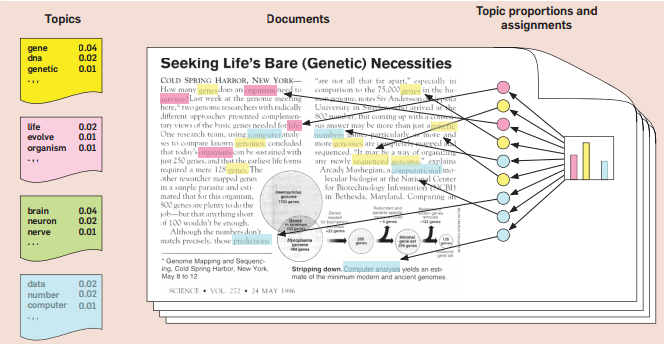
\includegraphics[scale=0.8]{topicmodel}
\caption{Simple topic modelling approach for a single article\cite{blei2012probabilistic}}.
\label{figure:example}
\end{center}
\end{figure*} 


\subsubsection{Topic Detection Model}
\label{topic detection:model}
\paragraph\textbf{Latent Dirichlet Allocation (LDA) Model}

LDA is a generative probabilistic model in which each document is modeled as a finite mixture over an underlying set of topics and each topic, in turn, is modeled as an infinite mixture over an underlying set of topic probabilities\cite{blei2003latent}. In other words, documents exhibit multiple topics and each topic is a distribution over a fixed vocabulary.
The LDA model can be briefly reviewed as follows:


Given an input corpus of $D$ documents with $K$ topics, each topic being a multinomial distribution over a vocabulary of  $W$ words, the documents are modeled by fitting parameters `${\Phi}$' and `${\Theta}$'. `${\Phi}$' is a matrix of size $D \times K$ in which each row is a multinomial distribution of document $d$  indicating the relative importance of words in topics. ${\Theta}$ is the matrix of size $W \times K$ with each column a multinomial distribution of topic $j$ and corresponds to the relative importance of topics in documents.

Given the observed words x = ${x_i}_j$, LDA inference is done by computing the
posterior distribution over the latent topic assignments z = ${z_i}_j$, the mixing proportions ${\Theta_j}$  and the
topics ${\Phi_k}$.  The inferencing is either done using variational bayesian methods or Gibbs sampling which involves integration and sampling of latent variables.
However, the simple LDA approach can take several days to run over a large corpora.


\paragraph\textbf{Distributed LDA Model}
 
The simple LDA method takes a long time for topic modeling which is why the distributed version suits large datasets such as ours. The data is partitioned across separate processors and inference is done in a parallel, distributed fashion. 

The Approximate Distributed LDA (AD--LDA) model as proposed by \cite{newman2009distributed} uses distributed computation where total dataset $D$ is distributed equally among multiple $P$ processors. Initialization involves data and parameters distribution to each processor and random assignment of topics so that each processor has its own copy of words $x_p$, topics $z_p$, word topic counts ${{{N_w}_k}_p}$ and topic counts ${{{N_k}_j}_p}$. 
The topic model inferencing then uses simultaneous local Gibbs sampling approach on each processor for a pre-decided number of iterations to reassign topic probabilities $z_p$, word topic ${{N_w}_k}_p$ and topic counts ${{N_k}_j}_p$.
Global update is performed after each pass by using a reduce-scatter operation on word topic count ${{N_w}_k}_p$ to get a single set of counts and obtain final topic assignments.
The model requires user set parameters before inferencing such as number of processors/threads for parallel sampling of data, number of iterations of Gibbs sampling, number of topics and Dirichlet parameters. 

\subsubsection{Topic Models Evaluation}

 Different topic models can be evaluated using the metric of ``Perplexity" which can be defined as how surprised a trained model is when given a held out test data. It has been used in \cite{newman2009distributed} and \cite{blei2003latent} for evaluating the topic detection models under different parameter settings. Perplexity can be calculated using the following formula:

$$Perplexity= \exp(-\dfrac{\text{Log Likelihood of held-out test set}}{\text{Number of tokens in held-out test set}})$$


Here, held-out test set refers to the fact that complete dataset is split into two parts: one for training and the other for testing. The test set is taken as the held-out set for which perplexity is calculated. The document mixture is learned using the training data and log probability of the test data containing unseen documents is computed using the model developed.

Perplexity is a decreasing function of the log likelihood of the unseen documents as can be seen from its formula and lower the perplexity, better is the topic model.

\subsubsection{Results}
\label{topic detection:result}

The AD-LDA model as described in \cite{newman2009distributed} and implemented in the Mallet\cite{McCallumMALLET} toolkit (known as PLDA model) is used for topic detection over the complete dataset of 14020 news articles. 
Several topic models are first evaluated with different parameter settings in order to pre-decide the number of iterations, processors and topics for the final topic model to be used.


%After training, parameter settings as number of topics varying from 10 to 100, number of iterations from 100 to 500 and number of processors from 1 to 8, the log likelihood of held-out test dataset is calculated along with number of tokens in it to obtain perplexity.

\begin{figure*}
\begin{center}
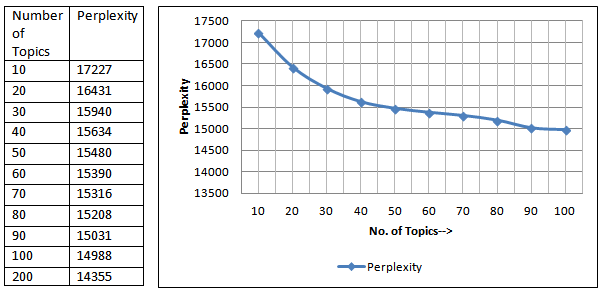
\includegraphics{topicperplex2}
\caption{Test Set Perplexity versus Number of Topics for a random $90-10$ split of the data. The maximum number of words in each topic is $20$, number of iterations $500$ and the number of processors $4$ for this experiment.}
\label{figure:perplex}
\end{center}
\end{figure*}

Perplexity is calculated by splitting the data into 90\% for training and rest 10\% for testing. 
Figure~\ref{figure:perplex} shows the variation of the test perplexity versus the number of topics for one random $90-10$ split of the data\footnote{We also vary the number of iterations from 100 to 500 and number of processors from 1 to 8 to study their effect on perplexity. However the number of topics is most influenced by perplexity and hence the other results are not presented here.}. The maximum number of words in each topic is set to $20$, number of iterations $500$ and the number of processors $4$ for this experiment. It exhibits a decreasing perplexity with increase in number of topics. Typically, the number of topics should be chosen as high as possible in order to consider a better model with low perplexity but the model with high number of topics also takes longer to run on a large dataset. The number of topics is set to a value from where further increase in number of topics does not lead to a large decrease in perplexity. We choose the number of topics as $30$ and $100$ and demonstrate their effect on the influential people detection.

From the various topic models and parameter settings, the variability in perplexity with respect to the number of topics has been found to be much greater than the variability due to the number of processors or number of iterations. This is why two values of number of topics are experimented further while number of processors and number of iterations are kept fixed. The number of iterations of Gibbs sampling still need to be above the typical burn-in period of $200$ which is why $500$ is chosen as the parameter value for number of iterations. Number of threads/processors is similarly taken as 4 as least training time is obtained with this parameter value. 

The two models from topic detection are thus used with following parameters:
\begin{enumerate}
 \item \textbf{30 Topics LDA Model} : Number of topics = 30, Number of iterations = 500, Number of threads=4
 \item \textbf{100 Topics LDA Model} : Number of topics = 100, Number of iterations = 500, Number of threads=4
\end{enumerate}
The first model takes 7.5 minutes for training while the second one takes 8.6 minutes.
The set of 30 topics obtained through the first model are illustrated in Table~\ref{table:topicwords} and the other model with 100 topics in Appendix Table~\ref{long}. Some of the topics words can be easily identified to belong to  the following topics: music performance, court events, elections and government and shipping.

Topic modeling gives as output, for each article in the dataset, a set of topics with their probability distribution score for the article. The topic with highest topic probability score is associated with each article in the dataset. 


\subsection{People Gazetteer Output }
\label{gaz:result}

The list of articles obtained for each person entity after application of PNER and highest scoring topic assigned to each article during Topic Detection are combined to obtain People Gazetteer. In each tuple of the gazetteer, a person entity gets associated with its list of articles where each article is further associated with its corresponding highest scoring topic.

Two people gazetteers are obtained, each corresponding to the two model settings of 30 Topics LDA Model and 100 Topics LDA Model, respectively. A snapshot of the people gazetteer using 30 Topics LDA Model can be seen in Figure~\ref{figure:gazette} where each person entity is followed by a document list consisting of a Document ID and its corresponding Topic ID. A similar people gazetteer is also obtained using 100 Topics LDA Model. Both People Gazetteers are further used in Chapter~\ref{chapter:influential people detection} for detecting and ranking influential person entities from them.
\begin{figure*}
\centering
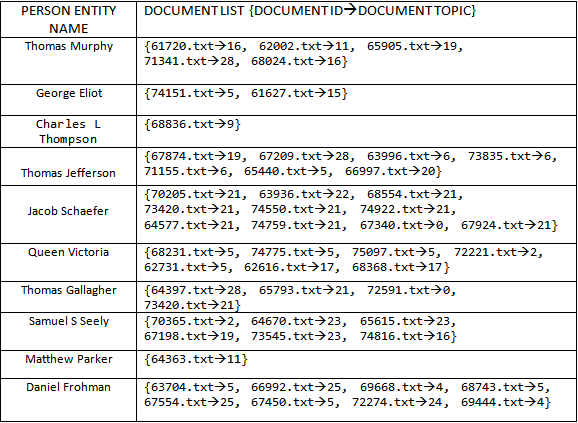
\includegraphics{gazetteer}
\caption{Snapshot of People Gazetteer with Person names, Document list of occurrence and their corresponding Topic ID}
\label{figure:gazette}
\end{figure*} 




% needed in second column of first page if using \IEEEpubid
%\IEEEpubidadjcol



% An example of a floating figure using the graphicx package.
% Note that \label must occur AFTER (or within) \caption.
% For figures, \caption should occur after the \includegraphics.
% Note that IEEEtran v1.7 and later has special internal code that
% is designed to preserve the operation of \label within \caption
% even when the captionsoff option is in effect. However, because
% of issues like this, it may be the safest practice to put all your
% \label just after \caption rather than within \caption{}.
%
% Reminder: the "draftcls" or "draftclsnofoot", not "draft", class
% option should be used if it is desired that the figures are to be
% displayed while in draft mode.
%
%\begin{figure*}
%\centering
%\includegraphics[width=2.5in]{myfigure}
% where an .eps filename suffix will be assumed under latex, 
% and a .pdf suffix will be assumed for pdflatex; or what has been declared
% via \DeclareGraphicsExtensions.
%\caption{Simulation results for the network.}
%\label{fig_sim}
%\end{figure}

% Note that IEEE typically puts floats only at the top, even when this
% results in a large percentage of a column being occupied by floats.
% However, the Computer Society has been known to put floats at the bottom.


% An example of a double column floating figure using two subfigures.
% (The subfig.sty package must be loaded for this to work.)
% The subfigure \label commands are set within each subfloat command,
% and the \label for the overall figure must come after \caption.
% \hfil is used as a separator to get equal spacing.
% Watch out that the combined width of all the subfigures on a 
% line do not exceed the text width or a line break will occur.
%
%\begin{figure*}
%\centering
%\subfloat[Case I]{\includegraphics[width=2.5in]{box}%
%\label{fig_first_case}}
%\hfil
%\subfloat[Case II]{\includegraphics[width=2.5in]{box}%
%\label{fig_second_case}}
%\caption{Simulation results for the network.}
%\label{fig_sim}
%\end{figure*}
%
% Note that often IEEE papers with subfigures do not employ subfigure
% captions (using the optional argument to \subfloat[]), but instead will
% reference/describe all of them (a), (b), etc., within the main caption.
% Be aware that for subfig.sty to generate the (a), (b), etc., subfigure
% labels, the optional argument to \subfloat must be present. If a
% subcaption is not desired, just leave its contents blank,
% e.g., \subfloat[].


% An example of a floating table. Note that, for IEEE style tables, the
% \caption command should come BEFORE the table and, given that table
% captions serve much like titles, are usually capitalized except for words
% such as a, an, and, as, at, but, by, for, in, nor, of, on, or, the, to
% and up, which are usually not capitalized unless they are the first or
% last word of the caption. Table text will default to \footnotesize as
% IEEE normally uses this smaller font for tables.
% The \label must come after \caption as always.
%
%\begin{table}[!t]
%% increase table row spacing, adjust to taste
%\renewcommand{\arraystretch}{1.3}
% if using array.sty, it might be a good idea to tweak the value of
% \extrarowheight as needed to properly center the text within the cells
%\caption{An Example of a Table}
%\label{table_example}
%\centering
%% Some packages, such as MDW tools, offer better commands for making tables
%% than the plain LaTeX2e tabular which is used here.
%\begin{tabular}{|c||c|}
%\hline
%One & Two\\
%\hline
%Three & Four\\
%\hline
%\end{tabular}
%\end{table}

% Note that the IEEE does not put floats in the very first column
% - or typically anywhere on the first page for that matter. Also,
% in-text middle ("here") positioning is typically not used, but it
% is allowed and encouraged for Computer Society conferences (but
% not Computer Society journals). Most IEEE journals/conferences use
% top floats exclusively. 
% Note that, LaTeX2e, unlike IEEE journals/conferences, places
% footnotes above bottom floats. This can be corrected via the
% \fnbelowfloat command of the stfloats package.







\section{Influential People Detection}
\label{influential:measure}

To measure influence in the newspaper environment and to compare and rank people as influential, we define an influence score measure called \textit{``Influential Person Index" (IPI)} corresponding to each person entity in the people gazetteer. To calculate IPI for each person entity, we first define the \textit{``Document Index" (DI)} to measure how each document in the person entity's associated list of documents affects his influence score.
Following subsections describe the parameters for calculation of DI and IPI of a person entity followed by the complete algorithm for detection of influential persons:

\subsection{Document Index (DI)}

The Document Index (DI) of an article in the people gazetteer helps to measure a person's influence score. Following parameters are considered for the calculation of this index:

\begin{enumerate}
\item \textbf{Normalized Document Length} (NDL)\\
Document Length affects the influence score in the sense that a longer news article in which a person entity occurs is deemed to be more important than a shorter one. It is defined as the number of tokens contained in a news article. Document Length is further normalized by dividing it with the maximum news article length (of 14020 articles in the dataset) to get Normalized Document Length as follows: 

$$NDL=\dfrac{\text{Document Length}} {\text{Maximum Document Length in the dataset}}$$


%\item[$\bullet$IDF]
%IDF is used as a parameter in the calculation of DI of a news article to give weight to the person entity's occurrence in the complete %dataset. It can be calculated as the number of news articles in which a person entity occurs in the complete dataset. It is %equivalent to the length of document list in the people gazetteer for each person entity.

\item\textbf{ Normalized Term Frequency} (NTF)\\
Term Frequency (TF) accounts for the number of occurrences of a person's name in a news article. The TF of the person name affects a document's influence score as a higher number of occurrences in the document makes it more important. TF is further normalized and calculated as follows:

\begin{center}
$NTF=	1	+\log	$(TF of person entity in current article)
\end{center}

\item \textbf{Number of similar articles} (NSIM)\\
This parameter is used in calculation of the DI by finding articles of similar topic in the document list. 
%The set of topics derived from a corpus can be used to answer questions about the similarity of words and 
%documents.
Two documents are considered similar if they belong to the same topics. For a document $d$ whose DI is to be calculated, we consider 

SIM= Number of articles with the same topic as that of $d$ in the document list of person entity.

This measure is normalized by dividing it with the number of total articles in the document list of the person entity as follows:

\begin{center}
$NSIM= \dfrac{\text{SIM}} {\text{Total number of articles in the person's document list}}$
\end{center}
NSIM can be said to be equivalent to the proportion of topic similar articles that any document $d$ has.

This parameter takes into account the effect of a document's score on a person's IPI when there exist several other documents of the same topic in the person's list. 


\end{enumerate}

DI for each document is a function of the above mentioned parameters and is calculated using the following formula :
\begin{center}

			$DI = w_a . NDL + w_b . NSIM + w_c . NTF $
\end{center}
where, $w_a$,$ w_b$ and $w_c$ are the weights associated with each of the parameters NDL, NSIM and NTF respectively.


DI is actually a heuristic measure of these three parameters where each of the parameters can be weighted as per dataset characteristics and user requirements. For example, a higher value to $w_a$ and lower to $w_b$ and $w_c$ indicates documents with longer lengths are considered more important for influencing a person's IPI. On the other hand, a higher value to $w_b$ and lower to $w_a$ and $w_c$ indicates a document with larger proportion of topic similar articles influences the person's IPI more suggesting assignment of high influence score to a person entity occurring repeatedly in a specific news topic.  

\subsection{Influential Person Index (IPI)}

Once DI is calculated for each document in a person's list, an index is calculated for the person entity in order to measure its influence in the news dataset and calculate its influential score. The ``Influential Person Index" defined for this purpose is calculated as follows:
		
\begin{center}
$IPI= max DI(d_1, d_2, ...,d_n)+ UniqT$
\end{center}

where , $max DI(d_1, d_2, ...,d_n)$ = Maximum Document Index of a document $d_i$ in a person entity's list of  $n$ articles, and
\begin{center} $UniqT = \dfrac{\text{Number of Unique Article Topics in a person entity's document list}}{\text{Total Number of Topics in the corpus}}$\end{center} 

The parameter $UniqT$  is used to account for the fact that a single person entity can be talked about multiple news topics in the news articles and to include its effect on the person entity's influence score. It is normalized by dividing it with the total number of topics as obtained during topic detection on all 14020 articles.

Ranking is done across each person category of the people gazetteer to obtain top most influential persons. For this, IPI for each person entity across the person categories are sorted in decreasing order to obtain the most influential person entities with highest IPI at the top.
  
\subsection{Procedure for finding influential persons}

Algorithm ~\ref{algorithm:3} depicts the procedure for measuring influence and ranking of influential people from the gazetteer. It starts with calculation of DI for each news article in a person's document list by calculating the required parameters of NDL, NSIM and NTF which are assigned 0 values initially. The respective weights $w_a$,$w_b$,$w_c$ are taken as inputs and multiplied with each parameter to get final DI score which is added to the list of DI scores $DIScoreList$. The list is sorted to find the maximum DI value among all news articles in the person's document list. The maximum DI score is then added to the UniqT parameter to get the final IPI for each person entity which are again stored and sorted to obtain a ranked list of influential person entities.  



\begin{algorithm}[!htb]
\caption{Procedure to calculate IPI and rank person entities based on it}
\label{algorithm:3}
\begin{algorithmic}
\Function {CalculateIPI}{}
  

%%%%%%DOUBT HERE.....
 \KwIn{$PeopleGazetter(Persons,(DocList,$}
\KwIn{$TopicList))$, $w_a$,$w_b$,$w_c$}
\KwResult{Ranked list of Person Name and IPI}  
 $NTF \leftarrow $0,  $NDL \leftarrow $0, $NSIM \leftarrow $0, $DI\leftarrow $0, $UniqT\leftarrow $0, $IPI\leftarrow $0\;  
  
    \For{(String PersonName : Persons)}
     {
	   \For{(String doc  : DocList)}
	{	
		$NTF=1+\log (GetPersonTF(doc))$;
		
$NDL=GetDocLength(doc)/GetMaxDocLength()$;

		$ NSIM=GetTopicSimilarArticles(doc,DocList)$;

		$DI=w_a . NDL+w_b . NSIM+ w_c . NTF$;
		
		$DIScoreList.add(DI)$;
 	 }
		$Sort(DIScoreList)$;

		$UniqT=GetUniqueTopics(Person,TopicList)$;

		$IPI=Max(DIScoreList)+UniqT$;

		$IPIScores.put(PersonName,IPI)$;
       }
	$Sort(IPIScores)$;

	$PrintPersonNameandMaxIPI(IPIScores)$;

\EndFunction
\end{algorithmic}
\end{algorithm}

\begin{table*}
\begin{center}
\begin{tabular}{|c|c|} \hline
Function Name & Description \\ \hline
GetPersonTF(doc) & Calculates TF of the person entity \\
 & in document $doc$ \\ \hline
GetDocLength(doc) & Calculates number of tokens in $doc$. \\ \hline
GetMaxDocLength() & Calculates maximum number of \\
& tokens in any document.\\ \hline
GetTopicSimilarArticles(doc,DocList) &  Calculates normalized number \\
& of topic similar articles for $doc$ in the $DocList$. \\ \hline
Sort(DIScoreList) & Sorts the $DIScoreList$ \\ \hline
Max(DIScoreList) & Finds the maximum score from $DIScoreList$. \\ \hline
GetUniqueTopics(Person,TopicList) & Calculates normalized unique \\
& topics for $Person$ in its $TopicList$. \\ \hline
Sort(IPIScores) & Sorts the $IPIScores$ by IPI values. \\ \hline
PrintPersonNameandMaxIPI(IPIScores) & Prints $Person$ name with its \\
& IPI in decreasing order of IPI value. \\ \hline
\end{tabular}
\end{center}
\caption{Description of the functions used in Algorithm~\ref{algorithm:3}}
\label{default}
\end{table*}%

\begin{figure*}
\begin{center}
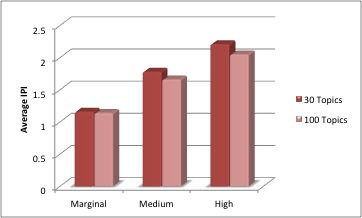
\includegraphics[scale=0.75]{IPIChart}
\end{center}
%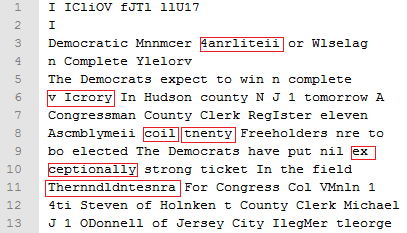
\includegraphics[scale=0.80]{ocr}
\caption{Comparison of the Average IPI for two ranked lists $L_1$ and $L_2$ using $30$ and $100$ topics respectively.}
\label{figure:IPI}
\end{figure*}



\section{Results}
\label{influential:results}
Two ranked influential person lists, namely L1 and L2 are obtained after calculation of IPI from the people gazetteer (developed in Chapter~\ref{chapter:people gazetteer}) using 30 Topics and 100 Topics LDA Model respectively. The weights $w_a$, $w_b$ and $w_c$ are all set to 1 to give equal importance to each of the parameters during calculation of DI and IPI. The statistics obtained from both lists with respect to each person category of the people gazetteer are shown in Table~\ref{table:stats}. 
It can be clearly observed from the table that Highly Influential Persons occur in most number of news articles on an average and with highest average term frequency followed by Medium Influential and Marginal Influential Persons.
Document Length need not always be too high for a person to be ranked higher as can be observed from the fact that average document length obtained for Marginally Influential People is high in spite of their Average IPI being low indicating that the varying number of similar articles for each document as well as its Term Frequency share also play an important part in measuring influence. Figure~\ref{figure:IPI} shows the average IPI from the two ranked lists -- it appears that the average IPI for highly influential people is more susceptible to changes in number of topics.

\begin{table*}
\begin{center}

    \begin{tabular}{|p{2cm}|p{2cm}|p{2cm}|p{2cm}|p{2cm}|}
    \hline
    \textbf{Person Category}  &  \textbf{Number of Person Entities}   & \textbf{Average Number of Documents}   &  \textbf{Average Document Length}	&  \textbf{Average Term Frequency}	\\  \hline
Marginal & 38066 & 1.04 & 2119.6 & 1.07 	\\ \hline
Medium & 344 & 5.75 & 1976.3 & 6.68  \\ \hline
High & 16 & 22.8 & 2971.5 & 29.870	 \\	\hline 
  \end{tabular}
  \end{center}
    \caption {Table illustrating average statistics for each Person Category of People Gazetteer across 2 Topic Models}
\label{table:stats}
\end{table*}


The following sections present comparison between the ranked influential person lists L1 and L2, some case studies and evaluation results:
 
\begin{table*}
\begin{tabular}{|p{2cm}|l|p{1.5cm}|p{1.5cm}|l|l|l|p{3cm}|l|l|}
\hline
Person Name    & IPI  & Number of Articles & Person Category & NDL  & NTF  & NSIM & TOPIC WORDS                                                          & UniqT & Rank \\ \hline
capt creeten   & 3.38 & 10                 & Medium          & 0.56 & 1.95 & 0.8  & mr court police judge justice case yesterday street district         & 0.06  & 1    \\ \hline
capt hankey    & 3.02 & 6                  & Medium          & 0.68 & 1.6  & 0.66 & club game team play football half ball left college back             & 0.06  & 2    \\ \hline
capt pinckney  & 2.93 & 3                  & Marginal        & 0.38 & 1.84 & 0.67 & man ho men night back wa room left house told bad                    & 0.03  & 3    \\ \hline
john macdonald & 2.85 & 3                  & Marginal        & 0.55 & 2.2  & 0    & great people life man women good country world american part         & 0.1   & 4    \\ \hline
john martin    & 2.82 & 12                 & Medium          & 0.56 & 1.6  & 0.5  & mr court police judge justice case yesterday street district witness & 0.17  & 5    \\ \hline
aaron trow     & 2.81 & 1                  & Marginal        & 0.7  & 2.07 & 0    & man ho men night back wa room left house told                        & 0.03  & 6    \\ \hline
mrs oakes      & 2.79 & 5                  & Medium          & 0.08 & 2.04 & 0.6  & street mrs mr avenue wife house miss yesterday years home            & 0.06  & 7    \\ \hline
buenos ayres   & 2.76 & 6                  & Medium          & 0.43 & 1.6  & 0.67 & white water indian black long found thu big dog time                 & 0.06  & 8    \\ \hline
alexander iii  & 2.74 & 31                 & High            & 0.24 & 2.04 & 0.29 & great people life man women good country world american part         & 0.16  & 9    \\ \hline
mr got         & 2.73 & 3                  & Marginal        & 0.56 & 1.47 & 0.67 & mr court police judge justice case yesterday street district witness & 0.03  & 10    \\ \hline
\end{tabular}
\caption{Table showing top 10 influential persons of List L1 detected from People Gazetteer with 30 Topics LDA model. Parameters NDL, NTF,NSIM and Topic Words belong to the maximum scoring DI in the person's document list.}
\label{table:30t}
\end{table*}

\begin{table*}
\resizebox{16cm}{!} {
\begin{tabular}{|p{2cm}|l|p{1.5cm}|p{1.5cm}|l|l|l|p{3cm}|l|l|}
\hline
Person Name    & IPI  & Number of Articles & Person Category        & NDL  & NTF  & NSIM & Topic Words                                                                 & UniqT & Rank \\ \hline
capt creeten   & 3.33 & 10                 & Medium     & 0.56 & 1.95 & 0.8  & mr police witness committee capt asked captain money inspector paid         & 0.02  & 1    \\ \hline
mrs martin     & 3.23 & 8                  & Medium     & 0.20 & 2.38 & 0.5  & mrs mr years wife home house ago woman city died                            & 0.02  & 2    \\ \hline
alexander iii  & 3.09 & 31                 & High     & 0.49 & 2.04 & 0.48 & emperor prince french alexander czar london nov government imperial russian & 0.07  & 3    \\ \hline
capt hankey    & 2.97 & 6                  & Medium    & 0.68 & 1.6  & 0.66 & game team football play half line ball back yale eleven                     & 0.02  & 4    \\ \hline
aaron trow     & 2.79 & 1                  & Marginal & 0.70 & 2.07 & 0    & day place long great water time feet found good men                         & 0.01  & 5    \\ \hline
john macdonald & 2.77 & 3                  & Marginal & 0.55 & 2.2  & 0    & people american man great country men world life good english               & 0.02  & 6    \\ \hline
mrs oakes      & 2.74 & 5                  & Medium     & 0.08 & 2.04 & 0.6  & mrs mr years wife home house ago woman city died                            & 0.02  & 7    \\ \hline
john martin    & 2.71 & 12                 & Medium     & 0.56 & 1.6  & 0.5  & mr police witness committee capt asked captain money inspector paid         & 0.05  & 8    \\ \hline
ed kearney     & 2.63 & 7                  & Medium     & 0.16 & 1.6  & 0.85 & won time race ran mile furlough half lo track fourth                        & 0.01  & 9    \\ \hline
caleb morton   & 2.61 & 1                  & Marginal & 0.70 & 1.9  & 0    & day place long great water time feet found good men                         & 0.01  & 10   \\ \hline

\end{tabular}}
\caption{Table showing top 10 influential persons of  List L2 detected from People Gazetteer with 100 Topics LDA model. Parameters NDL, NTF,NSIM and Topic Words belong to the maximum scoring DI in the person's document list.}
\label{table:100t}
\end{table*}
\subsection{Comparison Across Ranked Influential Person Lists }

The top 10 influential persons from List L1 and L2 detected from each of the people gazetteers are presented in Table ~\ref{table:30t} and ~\ref{table:100t} respectively.
It can be clearly seen from both the tables that the person category labels assigned during development of people gazetteer do not hold true after detection of influential persons. This suggests that the highly influential category people which were defined as person entities with more than 16 articles in the dataset might not necessarily be the most influential. The top 10 influential persons in both tables are dominated by Medium and Marginal category persons having considerably less number of articles of occurrence. This indicates the fact that number of articles of occurrence has not been given priority while measuring influence of a person entity. 
The statistics for top 10 influential people from both the tables also suggest that none of the measures of NDL, NTF or NSIM can be alone used to say whether a person entity is influential since these value do not decrease or increase consistently although the NTF measure does contribute most to the IPI of any person.

\newpage
The ranked influential lists L1 and L2 can be contrasted in terms of NSIM, UniqT and Topic Words since they vary across different number of topics and to see the effect of 30 and 100 Topics LDA Models on influential person detection.
 If NSIM (normalized number of topic similar articles) remains same in L1 and L2 during influential person detection from both the people gazetteers, then the same highest scoring article' DI is selected for calculation of IPI in both of them. This is why the parameters NDL (Normalized Document Length) and NTF (Normalized Term Frequency) remain same across both the lists. This can be seen for person like ``capt creeten", ``capt hankey", ``aaron trow" and "mrs oakes" in Tables ~\ref{table:30t} and ~\ref{table:100t}. But the value of UniqT for these persons decreases leading to decrease in their final IPI in the second table. This is because LDA model with higher number of topics (100) is used in this case due to which the proportion of unique topics becomes lower when NSIM does not change.
However, when the NSIM (normalized number of topic similar articles) value changes because of change in number of topics, a different article with maximum DI score can get selected leading to change in the values of NDL, NTF, UniqT and the final IPI. This causes a shift in the ranking of influential persons across the two lists and can be seen when the rank of ``alexander iii" in the first table moves from 9 to 3 in the second table. 
This indicates the fact that LDA Topic Model used affects the ranking of influential persons when number of topics are varied.

  \subsection{Case Studies}

Some of the topmost 10 influential person entities of lists L1 and L2  (Table ~\ref{table:30t} and ~\ref{table:100t}) identified from each person category of the 2 people gazetteers are discussed below: 
\begin{enumerate}

\item
Highly Influential Category- This category as defined in Section~\ref{ner:results} includes person entities influencing number of news articles greater than 16. However, only one person entity (``alexander iii") from this category occurs in the top 10 influential persons. The entry for ``alexander iii" has an IPI of 2.94 and 3.09 respectively in list L1 and L2 . The person entity occurs in 31 news articles with 5 and 7 different topics in each of the lists. The most common topic words associated with this person entity are: ``emperor prince french alexander czar london nov government imperial russian" indicating the importance of this entity in government related news topics. The 100 Topic LDA model increases the IPI value of this entity because the NSIM value increases (more number of similar topic articles talk about this person) and a longer article gets maximum DI score resulting in a high IPI value and improvement in the ranking from rank 9 in the first table to rank 3 in the second.

\item
Medium Influential Category- The top 10 influential entities from Tables ~\ref{table:30t} and ~\ref{table:100t} contain the most number of person entities from this person category. The person entity``capt creeten" has been ranked as highest influential (Rank 1) across both the tables. It occurs in 10 news articles with 9 of them belonging to the same topic indicating the person influencing news articles of high topic similarity. Some of the most common topic words for this entity include `` mr police witness committee capt asked captain money inspector paid" indicating the importance of this entity in a judicial or police related news topic.
Several persons from this category like ``mrs martin" , ``mrs oakes"  although identified among the top 10 influential persons but suffer from the problem of co-referred person names and named entity disambiguation as it is hard to identify which exact person they refer to due to lack of first names.
 
\item
Marginally Influential Category- Person entities belonging to this category have extremely low occurrence in news articles although the IPI of topmost influential entities belonging to this category are comparable to those in the other 2 categories.
Several person entities with low occurrences in news articles like ``aaron trow", ``caleb morton", ``john macdonald"  belong to this category. These entities in spite of occurring in very few articles (1 to 3) occur a large number of times in those articles with comparatively longer article length indicating the importance of these entities with respect to the articles they occur in. Since each of the features has been given equal weight during the calculation of IPI,  these person entities with high NDL and NTF have been identified among the top 10 influential persons. 
 The person entity ``mr got" ranked as a high influential person belonging to this category has actually been falsely detected as influential as the PNER seems to have misrecognized this entity as a person entity.  

\end{enumerate} 


\subsection{Evaluation}

Due to the unavailability of ground truth consisting of influential people in the newspaper archives from November-December 1894, there is no way to validate our results. 
To broadly evaluate our results, a simple web search query with the person entity's name in the context of 19th century was done on the Wikipedia website for the top 30 influential persons of Lists L1 and L2 detected from the people gazetteer with 30 Topics LDA and 100 Topics LDA Model respectively.

Among the top 30, 16 person entities from List L1 and 14 from List L2 were found to be influential and popular in the 19th century across topic categories like theatre, politics, government, shipping, etc. Some of these influential persons from Lists L1 and L2 found in Wikipedia are shown in Figure~\ref{figure:inf}. 

\begin{figure*}
\begin{center}
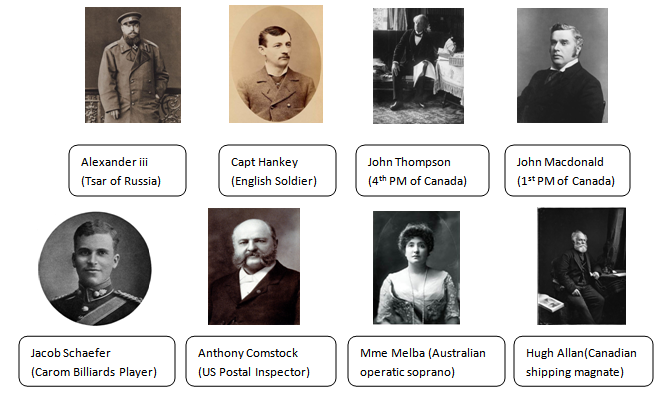
\includegraphics[scale=0.79]{ip}
\caption{Some of the top 30 influential persons obtained from the dataset and also found on Wikipedia during evaluation}
\label{figure:inf}
\end{center}
\end{figure*}


 Most of the false positives although influential in other respects but were not  influential `person' entities which can attributed to the incorrect PNER (Person Named Entity Recognition) on noisy OCR data.
 False positives are obtained for person entities  such as ``mr got" which is not a person entity at all and for entities such as ``ann arbor" and ``van cortlandt" which are in fact locations but got recognized as highly influential person entities.
 
 The ranked list of the top 30 influential persons with their IPI from Lists L1 and L2 can be seen in the Appendix (Table ~\ref{table:app1}.~\ref{table:app2}) where evaluation result for each person entity is also presented.


\section{Discussion}
\label{influential:discussion}


\begin{description}
\item[$\bullet$]\noindent
We used a linear combination of each of the parameters in calculation of DI and IPI and assigned equal values to the weights associated with each of them by not favoring any specific parameter. This is evident from the results which do not consistently favor any specific parameter. The parameters defined are based on heuristics and can be re-weighted according to user requirements or new parameters can be defined to do so. 

\item[$\bullet$]\noindent
The parameters for calculation of DI and IPI can also be learned by performing regression analysis using a manually developed sample of topmost influential people and obtaining the complete list of ranked influential people based on the learned parameters.

\item[$\bullet$]\noindent
The NDL(Normalized Document Length) parameter defined for calculation of DI is normalized using the maximum length of any document in the dataset. However, there might exist other ways of normalization of Document Length like using total number of tokens in a person entity's document list or total number of tokens in the complete dataset which can be experimented with according to the dataset.

\item[$\bullet$]\noindent
The topmost influential people contain several false positives also which occur not due to the influence measures defined but due to other factors discussed in Section ~\ref{gaz:discussion}. Several location and organization names have been misrecognized as person entities after performing Spelling correction and PNER resulting in false detection of some highly influential entities like ``van cortlandt", ``ann arbor" , ``sandy hook", etc.  There is also the problem of resolution of person name co-references in cases where persons like ``mrs martins" , ``mrs oakes", etc. have been recognized as influential.  

\item[$\bullet$] \noindent
The choice of parameters for topic detection also affects the detection of influential people which is evident from the fact that we get different ranking of influential people for the two different LDA Topic model settings used. 

\end{description}

\section{Conclusion}

The problem of finding influential people from historical OCR news repository has been studied in this research. In studying this novel problem, our main aim was to develop a complete solution framework for this problem and present insights from the results obtained.
 We made novel contributions to the problem solution by implementing an evaluation algorithm for measuring accuracy of spell correction on dataset, developing a people gazetteer for facilitating the process of influential people detection and finally defining parameters and measures in the newspaper community to obtain the ranked list of influential people.
Spelling correction algorithms with improved accuracy can certainly improve the influential persons results as well as use of a Named Entity Recognizer that can resolve co-referred person name issues in noisy OCR text.
Topic detection algorithms also need to be designed to enable them to deal with noisy OCR text in a better manner as some of the topics we obtained using LDA came out to be garbled and were difficult to understand in order to perform human-assigned manual labeling on them and use them further for finding similarity across articles.
We didn't consider Named Entity Disambiguation into account while developing the people gazetteer for detection of influential people which is a difficult problem in itself since it is hard to disambiguate among persons with similar names that can occur in multiple topic related articles in newspapers. The problem still requires research with probably better spelling correction, named entity recognition, topic detection algorithms and stricter measures of calculation of influence score and ranking of influential persons.

 The parameters we defined for measuring influence scores of persons in news articles are based on heuristics and can be re-weighted according to user requirements or new parameters can be defined based on the characteristics of an OCR newspaper dataset making it an open research problem.

Non-heuristic based estimation for finding influential persons can also be done using optimization approaches such as unsupervised multiple instance clustering\cite{zhang2009m3ic}. This approach can be used to cluster person entities into ``influential" or ``non-influential" by considering each person entity as a bag with articles of their occurrence as the instances for each bag. It is a combination of Constrained Concave-Convex Procedure and  Cutting Plane method with faster convergence. Such a method can avoid choosing of parameter weights, biasing of results with respect to any specific parameter and decide which article plays a role in determining whether a person is influential or not.

% if have a single appendix:
%\appendix[Proof of the Zonklar Equations]
% or
%\appendix  % for no appendix heading
% do not use \section anymore after \appendix, only \section*
% is possibly needed

% use appendices with more than one appendix
% then use \section to start each appendix
% you must declare a \section before using any
% \subsection or using \label (\appendices by itself
% starts a section numbered zero.)
%



% references section
% can use a bibliography generated by BibTeX as a .bbl file
% BibTeX documentation can be easily obtained at:
% http://www.ctan.org/tex-archive/biblio/bibtex/contrib/doc/
% The IEEEtran BibTeX style support page is at:
% http://www.michaelshell.org/tex/ieeetran/bibtex/
\bibliographystyle{IEEEtran}
% argument is your BibTeX string definitions and bibliography database(s)
\bibliography{aayushee}

% <OR> manually copy in the resultant .bbl file
% set second argument of \begin to the number of references
% (used to reserve space for the reference number labels box)
%\begin{thebibliography}{1}

%\bibitem{IEEEhowto:kopka}
%H.~Kopka and P.~W. Daly, \emph{A Guide to {\LaTeX}}, 3rd~ed.\hskip 1em plus
 % 0.5em minus 0.4em\relax Harlow, England: Addison-Wesley, 1999.



%\appendices
%Appendix one text goes here.

% you can choose not to have a title for an appendix
% if you want by leaving the argument blank
%\section{}
%Appendix two text goes here.

\begin{table*}
\centering
\begin{tabular}{|l|l|p{3cm}|p{3cm}|}
\hline
\textbf{Person Name}      & \textbf{IPI}      & \textbf{Whether found on Wikipedia} & \textbf{Comments}                                     \\ \hline
capt creeten     & 3.380151 & no                 & spelled incorrectly;capt creedon \\ \hline
capt hankey      & 3.022371 & yes                &                                      \\ \hline
capt pinckney    & 2.933288 & yes                &                                      \\ \hline
john macdonald   & 2.854389 & yes                &                                      \\ \hline
john martin      & 2.827969 & yes                &                                      \\ \hline
aaron trow       & 2.814171 & yes                & fictional character                  \\ \hline
mrs oakes        & 2.791536 & no                 & false positive                       \\ \hline
buenos ayres     & 2.767399 & no                 & location name                            \\ \hline
alexander iii    & 2.742552 & yes                &                                      \\ \hline
mr got           & 2.736363 & no                 & false positive                       \\ \hline
mrs martin       & 2.719383 & no                 & false positive                       \\ \hline
ann arbor        & 2.681657 & no                 & location name                            \\ \hline
caleb morton     & 2.63808  & no                 & fictional character                  \\ \hline
anthony comstock & 2.633381 & yes                &                                      \\ \hline
toledo ann arbor & 2.610495 & no                 & location name                            \\ \hline
john thompson    & 2.609841 & yes                &                                      \\ \hline
nat lead         & 2.594452 & no                 & false positive                       \\ \hline
ed kearney       & 2.543152 & yes                & name of horse                        \\ \hline
van cortlandt    & 2.533131 & no                 & location                             \\ \hline
louis philippe   & 2.523525 & yes                &                                      \\ \hline
mrs talboys      & 2.522888 & yes                & fictional character                  \\ \hline
jim hooker       & 2.500915 & yes                & false positive                       \\ \hline
marie clavero    & 2.497384 & no                 & false positive                       \\ \hline
father watson    & 2.450817 & no                 & false positive                       \\ \hline
james mccutcheon & 2.431448 & no                 & part of an organization name                      \\ \hline
hugh allan       & 2.4287   & yes                &                                      \\ \hline
william i        & 2.4222   & yes                &                                      \\ \hline
marie antoinette & 2.40731  & yes                &                                      \\ \hline
schmitt berger   & 2.396639 & no                 & spelled incorrectly;max f schmittberger                       \\ \hline
jacob schaefer   & 2.392976 & yes                &                                      \\ \hline
             
\end{tabular}
\caption{Table representing top 30 influential person entities detected from people gazetteer with 30 Topics LDA Model along with evaluation results and comments.}
\label{table:app1}
\end{table*}


\begin{table*}
\centering
\begin{tabular}{|l|l|p{3cm}|p{3cm}|}
\hline
\textbf{Person Name}      & \textbf{IPI}      & \textbf{Whether found on Wikipedia} & \textbf{Comments}                                     \\ \hline
capt creeten & 3.333485 & no & spelled incorrectly; capt creedon \\ \hline
mrs martin & 3.23105 & no & false positive \\ \hline
alexander iii & 3.090361 & yes &  \\ \hline
capt hankey & 2.975704 & yes &  \\ \hline
aaron trow & 2.790838 & yes &  \\ \hline
john macdonald & 2.774389 & no &  \\ \hline
mrs oakes & 2.744869 & no & false positive \\ \hline
john martin & 2.711302 & yes &  \\ \hline
ed kearney & 2.629342 & yes & name of horse \\ \hline
caleb morton & 2.614746 & no & fictional character \\ \hline
john ward & 2.57499 & yes &  \\ \hline
nat lead & 2.571118 & no & false positive \\ \hline
mrs talboys & 2.499555 & yes & fictional character \\ \hline
buenos ayres & 2.490502 & no & location \\ \hline
van cortlandt & 2.490169 & no & location \\ \hline
john thompson & 2.482063 & yes &  \\ \hline
louis philippe & 2.476858 & yes &  \\ \hline
marie clavero & 2.474051 & no & false positive \\ \hline
hardy fox & 2.449248 & no &  \\ \hline
mme melba & 2.415785 & yes &  \\ \hline
charles weisman & 2.405938 & no & false positive \\ \hline
hugh allan & 2.405367 & yes &  \\ \hline
mr got & 2.389697 & no & false positive \\ \hline
schmitt berger & 2.373305 & no & spelled incorrectly \\ \hline
phil king & 2.363644 & yes &  \\ \hline
henry a meyer & 2.350396 & yes &  \\ \hline
north orlich & 2.348236 & no & false positive \\ \hline
james mccutcheon & 2.338115 & no & part of organization name \\ \hline
gen porter & 2.330658 & yes &  \\ \hline
miller hageman & 2.327831 & no &  \\ \hline
\end{tabular}
\caption{Table representing top 30 influential person entities detected from people gazetteer with 100 Topics LDA Model along with evaluation results and comments.}
\label{table:app2}
\end{table*}



% use section* for acknowledgment
\ifCLASSOPTIONcompsoc
  % The Computer Society usually uses the plural form
  %\section*{Acknowledgments}
\else
  % regular IEEE prefers the singular form
  %\section*{Acknowledgment}
\fi


%The authors would like to thank...


% Can use something like this to put references on a page
% by themselves when using endfloat and the captionsoff option.
\ifCLASSOPTIONcaptionsoff
  \newpage
\fi



% trigger a \newpage just before the given reference
% number - used to balance the columns on the last page
% adjust value as needed - may need to be readjusted if
% the document is modified later
%\IEEEtriggeratref{8}
% The "triggered" command can be changed if desired:
%\IEEEtriggercmd{\enlargethispage{-5in}}



% biography section
% 
% If you have an EPS/PDF photo (graphicx package needed) extra braces are
% needed around the contents of the optional argument to biography to prevent
% the LaTeX parser from getting confused when it sees the complicated
% \includegraphics command within an optional argument. (You could create
% your own custom macro containing the \includegraphics command to make things
% simpler here.)
%\begin{IEEEbiography}[{\includegraphics[width=1in,height=1.25in,clip,keepaspectratio]{mshell}}]{Michael Shell}
% or if you just want to reserve a space for a photo:

%\begin{IEEEbiography}{Michael Shell}
%Biography text here.
%\end{IEEEbiography}

% insert where needed to balance the two columns on the last page with
% biographies
%\newpage

% You can push biographies down or up by placing
% a \vfill before or after them. The appropriate
% use of \vfill depends on what kind of text is
% on the last page and whether or not the columns
% are being equalized.

%\vfill

% Can be used to pull up biographies so that the bottom of the last one
% is flush with the other column.
%\enlargethispage{-5in}



% that's all folks
\end{document}


